\setcounter{figure}{0}

\section{16th April 2023: Are You Ready?}
\subsection*{Text: Revelation 19:1-10}
  \begin{quote}
    [1] After this I heard what seemed to be the loud voice of a great multitude in heaven, crying out,

    “Hallelujah!
    Salvation and glory and power belong to our God,
    [2]     for his judgments are true and just;
    for he has judged the great prostitute
        who corrupted the earth with her immorality,
    and has avenged on her the blood of his servants.”


      [3] Once more they cried out,

    “Hallelujah!
    The smoke from her goes up forever and ever.”


    [4] And the twenty-four elders and the four living creatures fell down and worshiped God who was seated on the throne, saying, “Amen. Hallelujah!” [5] And from the throne came a voice saying,

    “Praise our God,
        all you his servants,
    you who fear him,
        small and great.”


    [6] Then I heard what seemed to be the voice of a great multitude, like the roar of many waters and like the sound of mighty peals of thunder, crying out,

    “Hallelujah!
    For the Lord our God
        the Almighty reigns.
    [7] Let us rejoice and exult
        and give him the glory,
    for the marriage of the Lamb has come,
        and his Bride has made herself ready;
    [8] it was granted her to clothe herself
        with fine linen, bright and pure”—


    for the fine linen is the righteous deeds of the saints.

    [9] And the angel said to me, “Write this: Blessed are those who are invited to the marriage supper of the Lamb.” And he said to me, “These are the true words of God.” [10] Then I fell down at his feet to worship him, but he said to me, “You must not do that! I am a fellow servant with you and your brothers who hold to the testimony of Jesus. Worship God.” For the testimony of Jesus is the spirit of prophecy.
  \end{quote}
\subsection*{Notes}
\begin{itemize}
  \item{Recap: the bird's eye view of the book of Revelation is that there is
  a prologue and another chunk.  The prologue is the christophany, which
  includes the letters to the seven churches.  The other chunk can be divided
  into three sections (based on Pastor Ronnie's analysis):
  \begin{itemize}
    \item{Church age (this is where all the judgement is, the seven seals and trumpets and bowls)}
    \item{The second coming of Christ (the milennium age)}
    \item{New heavens and new Earth}
  \end{itemize}
  Pastor Ronnie said he is pre-mil lol.  The heavenly worship in chapter 4
  and the marriage supper of the lamb helps to interpret the text that is
  sandwiched in the middle.}
  \item{Three points for today:
  \begin{itemize}
    \item{Worship}
    \item{Worthy}
    \item{Watchful}
  \end{itemize}}
  \item{Recall the heavenly worship in chapter 4.  We have all the creatures
  glorifying God.  Why is there still chaos in the world now?  Chapter 4 is a
  reminder that the chaos in the world right now is not God's plan for the
  creation.  Sin is the thing that leads to the chaos, and sin must be dealt
  with.  And sin is dealt with in chapter 5 and beyond, through the Lamb.}
  \item{Babylon in the past symbolised the Roman empire, but not just the
  Roman empire specifically, but Babylon in general symbolises all of the
  world powers (secular or religious) that opposes God.}
  \item{First point on worship: in our text today, we have the great
  multitude in heaven praising God for judging Babylon.  Question: are the
  multitude praising God because Babylon is fallen, or are the multitude
  praising God because His judgements are faithful and true?  It is easy to
  praise and worship God when God executes judgment on the oppressors, even
  the pagans can do this (e.g the folk chinese obsession with Justice Bao).
  But it is difficult to praise and worship God when God seems to be silent
  in the midst of oppression.  Yet we must still remember that God is
  faithful and true, and in fact God is eternally faithful and true.  And God
  being faithful and true is our reason for worshipping him.  God will
  eventually judge evil, even if he seems silent at the moment.  God is
  unlike human judges, God being omnipotent and omniscient, knows the best
  time to do justice to everyone.  If we believe this, then we can worship
  God even in trials.}
  \item{The bride here refers to two possibilities:
  \begin{itemize}
    \item{The universal church of all believers.}
    \item{The saints who have been martyred for Jesus' sake.}
  \end{itemize}
  % In chapter 7, the identity of God's people has been established; God's
  % people are all who have been redeemed by Christ and sealed by God's Spirit.
  Pastor Ronnie argues that the bride here refers to the latter, but I don't
  agree with him lol.  His argument was that the idea of all believers being
  clothed with fine linen (which is the righteous deeds of the saints) goes
  against the protestant doctrine of justification by the imputation of
  Christ's righteousness onto the believers.  But my POV is that since those
  who are justified will eventually be sanctified and glorified, and if we
  remember that the righteous deeds of the saints are done through the Holy
  Spirit, then there is no real issue with God clothing ALL the saints with
  the fine linen since their righteous deeds are empowered by Him anyway!
  There is no risk of pelagianism.  Anyway the scene here is not a
  courtroom, it is a marriage, hence there is no reason to insist so strictly
  on the language of justification by the imputation of Christ's
  righteousness.  Let me check the commentaries I have...}
  \item{Ok moving on, as the angel who judged Babylon mentioned, there will
  be no more marriages in Babylon (marriages were one of the most joyous
  occasions in ancient days).  In contrast, there is a marriage in heaven.
  This is a contrast between those who commit immorality and God's people!}
  \item{OK I lazy to type liao. Oof. Sorry Ps Ronnie. I got stuck at the part about the bride.}
  \item{\begin{figure}[H]
    \centering
    % 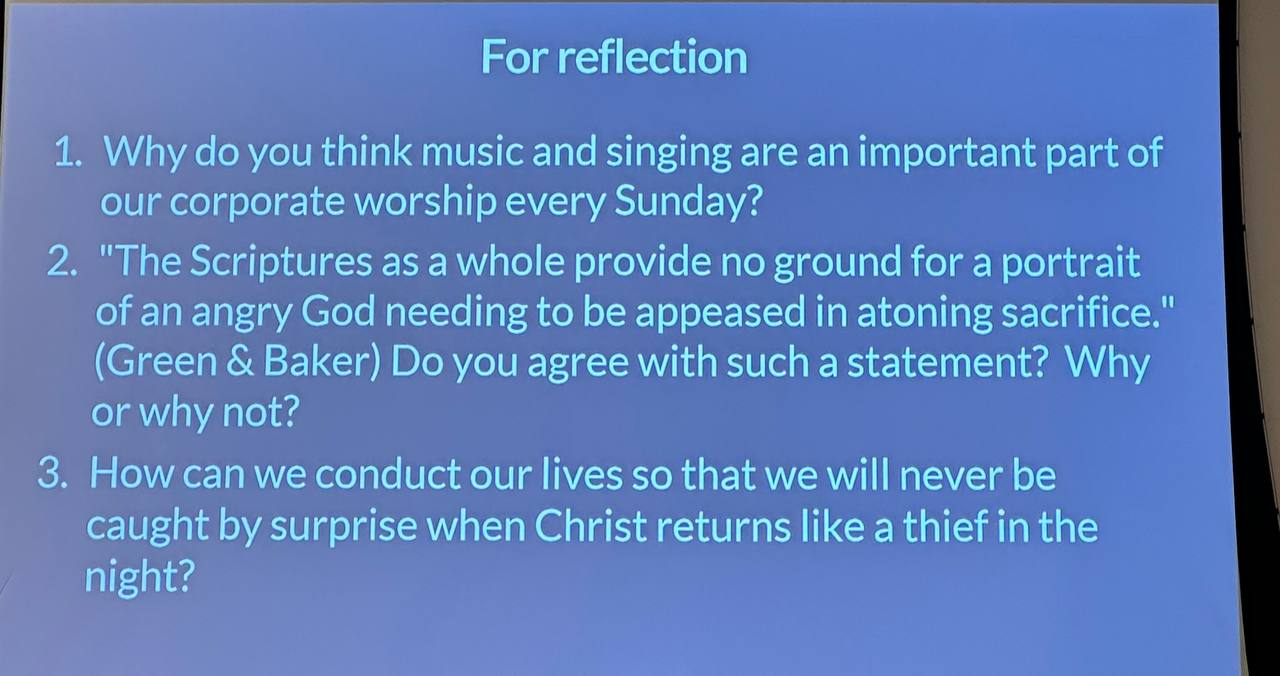
\includegraphics[width=0.8\textwidth, trim={0cm 0cm 0cm 0cm},clip]{Figures/marSermon4Reflections.jpg}
    \includegraphics[width=0.8\textwidth, trim={0cm 0cm 0cm 0cm},clip]{example-image-a}
    \caption[]{Reflection questions for this sermon}
    \label{}
  \end{figure}}
\end{itemize}